     %%%%%%%%%%%%%%%%%%%%
     %                  %
     %  capitolo1.tex   %
     %                  %
     %%%%%%%%%%%%%%%%%%%%

\section{Sviluppo dell'applicativo}

\subsection{Obiettivi}
L' obiettivo del software è quello di realizzare un applicativo che esegua \textit{model based tracking} \ref{modelTracking} sulla base di un video passatogli come ingresso. Più nel dettaglio l'applicazione esegue il tracciamento tramite il filtro di Kalman \cite{kalman-intro} e il ConDensaTion \cite{kalman-condense}, in maniera tale da poter confrontare le prestazioni dell' uno e dell'altro.\\
Altri requisiti funzionali sono quelli di:

\begin{itemize}
 \item  fare scegliere all'utente l'oggetto da tracciare in caso di tracking multiplo: in questo caso il software si ferma sul primo frame del video, dando possibilità di scegliere l'oggetto di cui si vuol fare il tracciamento. Per migliorare la selezione di un oggetto, vengono evidenziati dei un puntini gialli in corrispondenza del blob identificato. Vedi figura \ref{fig:scelta2blob}

\item tracciare a video l'andamento dei due algoritmi, evidenziandoli con colori differenti; visualizzare un' ellissi per ogni algoritmo che indichi la varianza del vettore di stato per quel tipo di tracking.

\item fornire un output razionalizzato su terminale e su filesystem per verificare rispettivamente la corretta esecuzione degli algoritmi e per avere un riscontro finale sulle performance e l'accuratezza di ognuno. Successivamente parsare i suddetti file per una rappresentazione grafica dell'accuratezza dei due metodi di tracking.

\item progettare e realizzare l'applicazione in maniera tale che possa essere compilata ed eseguite su piattaforme diverse.


\end{itemize}

I dettagli implementativi di questi punti sono rimandati alla sottosezione  \ref{ControlFlow}

\begin{figure}[hb]
\centering
	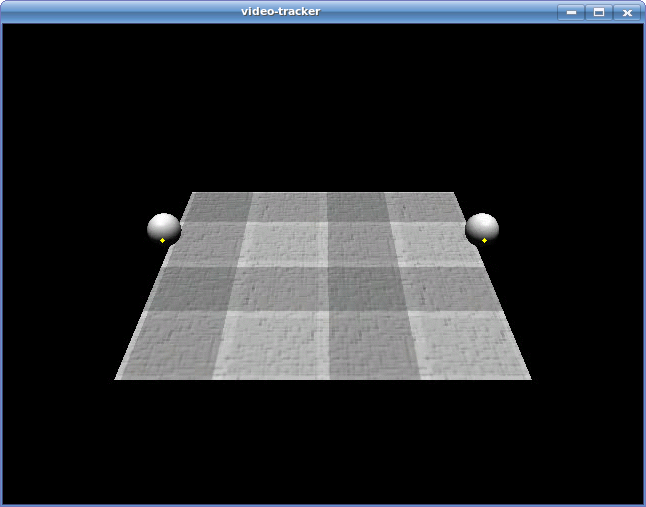
\includegraphics[scale=0.5]{doppiascelta.png}
\caption[Esempio di scelta tra due blob]{\textit{Esempio di scelta tra due blob su tracking multiplo: l'utente ha la possibilità di sccegliere su quale blob effettuare il tracciamento semplicemente cliccando vicino ad uno dei punti gialli. Il Sistema automaticamente selezionerà il blob più vicino attraverso il calcolo della distanza euclidea}\label{fig:scelta2blob}}
\end{figure}


\'E bene sottolineare che il video in ingresso possiede delle restrizioni: infatti affinchè il \textit{background subtraction} lavori in maniera ottima, è necessario che il video:
\begin{itemize}
 \item possieda semper uno sfondo fisso o che comunque non vari durante la ripresa. Cambiare sfondo sarrebbe come rinizializzare l'agoritmo per il detecting dei blob.
\item possieda un numero ( $n > 40 $ ) di frame inziale che mostrino solo il background per facilitare il calcolo della \textit{ground truth}, cioè del blob osservato da cui prendere le misure per i due algoritmi.
\item sia stato registrato da una postazione fissa e quindi che la telecamera di ripersa non introduca nel video un moto relativo.
 \end{itemize}

Qualsiasi video che rispetta questi tre vincoli è considerato non solo adeguato, ma ottimale per effettuare il tracking con la nostra applicazione.




%ingresso video fatto in un certo modo (sfondo fisso, tot frame di background iniziale, telecamera fissa)

%uno o + oggetti in moto

%permette di selezionare QUALE oggetto seguire, farne il tracciamento reale, ottenere le predizioni secondo k e c, e raccoglierne dati e risultati per la realizzazione di grafici

%intro utilizzo librerie utilizzate intel openCV
\subsection{Librerie Intel OpenCV}
Per svilluppare l'applicazione sono state utilizzate le libreria \textit{OpenCV}, emergente nel campo della \textit{computer vision}  e sviluppata da Intel sotto una licenza di tipo OpenSource, compatibile con la GNU GPL.
\'E bene però prima fare chiarezza sull'uso e lo scopo di queste librerie.\\
La capacità di interpretare ed utilizzare correttamente le informazioni acquisite da una videocamera o fotocamera attualmente presenta molti problemi insoluti. Convertire un’immagine in informazioni “oggettive” astraendone il contenuto dalla pura rappresentazione luminosa, sebbene sia un’operazione banale per un cervello umano adulto è, a tutt’oggi, un problema di elevata complessità per un sistema automatico.
Oltretutto il campo di ricerca è evidentemente molto giovane, con meno di trent’anni di esperienza. In quest’ottica si inserisce la necessità di una base comune di potenti strumenti analitici, primo dei quali una \textbf{libreria} che raccolga le funzionalità degli algoritmi più utilizzati e citati in letteratura, oltre che una serie di formati di rappresentazione dei dati secondo standard aperti e condivisi.\\
Le librerie OpenCV (Open Source Computer Vision) nascono appunto a questo scopo; lo sviluppo prende le mossa da un gruppo di ricerca sponsorizzato da Intel. E’ infatti parzialmente basata sulla \textit{Intel Image Processing Library (IPL)}: tale prodotto è oggi integrato nella libreria commerciale IIPP (Intel Integrated Performance Primitives), con cui conserva piena compatibilità e che può eventualmente rendere disponibili un completo ventaglio di funzioni più specifiche.\\
Tra i punti di forza sottolineiamo inoltre la politica di licenza utilizzata, in stile BSD e definita nella ``Intel License Agreement For Open Source Computer Vision Library'', completamente compatibile con la licenza GPL. A grandi linee questo permette una libera ridistribuzione sia in forma sorgente che binaria, anche all’interno di prodotti commerciali, a condizione di mantenere le note di copyright e di non utilizzare il nome Intel a scopo promozionale di prodotti derivati.\\
Inoltre un' altra potenzialità offerta è la caratteristica di essere \textit{cross-platform}: cioè possono essere compilate e usate sia sotto sistema operativo Microsft Windows che GNU/Linux. Questa caratteristica le rende molto appetibili per i requisiti di portabilià che ci eravamo prefissi di raggiungere.\\ Da notare che le librerie sono scritte in linguaggio C e non fanno uso quindi di un linguaggio orientato agli oggetti.

\subsubsection{Aree funzionali delle librerie}
Si vuol chiarire subito un fatto che può essere causa di equivoci: con il termine ``libreria grafica'' infatti si identificano genericamente almeno tre famiglie di librerie, i cui scopi sono sostanzialmente differenti:
\begin{enumerate}
 \item  I Toolkit, ovvero librerie di primitive per la creazione di oggetti grafici di interfaccia (finestre, icone, bottoni,ecc). Parzialemente ricoperto in OpenCV dalle HighGui.
\item Librerie di rendering e multimedia, come DirectX e OpenGL, orientate alla massima performance nella creazione di effetti poligonali o vettoriali. L’utilizzo più comune è teso all’ottenimento di elevate prestazioni    grafiche sfruttate ad esempio nei videogiochi o nelle applicazioni multimediali.
\item  Librerie di gestione hardware grafico, come digitalizzatori e frame-grabber. Pur includendo tipicamente una base di funzioni di trattamento sono generalmente da considerarsi come API dei relativi driver hardware.
\end{enumerate}

Le OpenCV, pur includendo alcune funzionalità tipiche di ciascuna delle famiglie citate \footnote{vedi esempio delle HighGui}, non fanno parte di nessuno di questi gruppi. L’utilizzo primario è infatti quello collegato alla visione artificiale, il cui problema principale, come già visto, è quello di estrarre da immagini/video dati significativi, trattabili in modo automatico. Tale campo di studio trova le sue applicazioni più comuni nella robotica, nei sistemi di  videosorveglianza evoluti e nei sistemi di monitoraggio e sicurezza, oltre che in ogni sistema di archiviazione automatica di informazioni visive.\\
La libreria include attualmente più di 300 funzioni, che coprono le più svariate esigenze di trattamento di immagini, comprese funzioni matematiche ottimizzate (elevamento a potenza, logaritmi, conversioni cartesiane-polari, ecc.) ed  un completo pacchetto di algebra matriciale, sviluppato funzionalmente al resto del sistema.\\

La principale categoria di uso rimane comunque il processing di tipo real-time su immagini e video. \\
Una panoramica generale delle librerie comprende questi aspetti della computer vision:
\begin{enumerate}
\item Human-Computer Interface (HCI)
\item Object Identification
\item Segmentation and Recognition
\item Face Recognition e Gesture Recognition
\item Motion Tracking  riferimento al nostro progetto
\end{enumerate}

%descrivere un po queste aree e dove si usano noi nel nostro progetto.




\subsubsection{Riferimenti}

Come molti progetti opensource in maturazione \footnote{La versione 1.0 ufficiale è stata rilasciata nel tardo 2006; parte del progetto è stato scritto con librerie in beta testing} è stata carente la parte che riguarda la documentazione. Nonostante la presenza di un colosso alla spalle e di una struttura basata sul modello wiki, la documentazione ufficiale in pdf e html, anche se facilmente fruibile, non è stata sufficiente per colmare le lacune iniziali. Per questo motivo è stato effettuato un grosso lavoro di studio per capire il funzionamento del toolkit OpenCv, che spesso è terminato con la ricerca di documentazione in website asiatici, dove sembra che queste librerie siano molto gradite.\\
Alcuni riferimenti importanti per OpenCV:
\begin{itemize}
 \item \htmladdnormallink{Sito web ufficiale}{http://www.intel.com/technology/computing/opencv/index.htm}
\item \htmladdnormallink{Portale di wiki}{http://opencvlibrary.sourceforge.net}
\item \htmladdnormallink{ OpenCv - Groups Community}{http://tech.groups.yahoo.com/group/OpenCV/}
\end{itemize}

 
\subsection{Control Flow del programma}\label{ControlFlow}
%intro del ciclozzo FOR e che cosa viene fatto in ordine con l'acquisizione frame/frame del video
Come citato precedentemente, si va ora a evidenziare quelli che sono stato gli accorgimenti tecnici per implementare il nostro software di comparazione tra Kalman e Condensation.\\
Si cercherà di non riportare tutto il codice sorgente, ma di evidenziare solo spezzoni di esso, che possono fornire preziose informazioni sulla struttura. \'E bene sottolineare che in linea con le OpenCV, la parte principale del software non è stata sviluppata secondo il paradigma Object Oriented, ma si è usato la razionalizzazione delle strutture dati in classi solo quando necessario.
Il nucleo centrale dell' applicazione è il \textbf{ciclo for} che dipende dalla lunghezza del video da analizzare. Ogni passo computazione verrà fatto in \textbf{modalità online}, cioè ad ogni passo dentro il ciclo stesso in maniera incrementale. Quindi in questo senso nessuno dei passi che andiamo a eseguire per fare il tracking risulta avere priorità su altri. \footnote{Per meglio spiegare gli effetti del metodo online si suppone di effettuare fuori dal cicolo il background subtraction su tutto il video e una volta finito questo passare all'analisi. Così facendo si appesantisce tutto l'algoritmo di calcolo e si dà una lunga attesa lato utente} \\

\newpage

I passi effettuati sono i seguenti:
\begin{itemize}
\item Apertura del video e ottenimento delle informazioni
\item Ciclo su tutti frame del video
\item Background Subtraction
\item Aggiornmaneto di Kalaman e Condensation
\item Rappresentazione dei risultati 
\end{itemize}

Nel listato di pseudo codice sottostante è riprotato l'idea dell' andamento dell'applicativo. 


\lstset{language=c++}
\lstset{commentstyle=\emph}
\begin{lstlisting}[frame=l,caption=Nucleo dell'Applicazione - execute.cpp ,breaklines=true,basicstyle=\small]{Nucleo dell'Applicazione - execute.cpp}

void execute( file ){

	video = captureFromAvi( file )
	
	initBackgroundSubtraction( video )

	for( int fr = 1; frame = captureNextFrame( video ), fr++ ){
	
		updateBackgroundSubtraction( frame )
		
		if ( frame == FIRST_FRAME){
			
			blobs = getBlobSelectedFromUser( frame )
	
			initKalman( blobs );
			
			initCondensation( blobs );
		}
	
		updateKalman();
		updateCondensation();
	}
}



\end{lstlisting}

Successivamente analizzeremo solo alcuni dei precedenti \textit{steps} elencati.

\subsubsection{Back subtraction}
%realizzazione online del backsub, librerie eccetera
L'idea di base del \textit{Background Subtraction}  è quella di identificare il livello di background per un determinato video, segmentando ogni frame in altri due frames chiamati rispettivamente:

\begin{itemize}
\item Foreground Mask
\item Background Mask
\end{itemize}

\begin{figure}[p]
\centering
	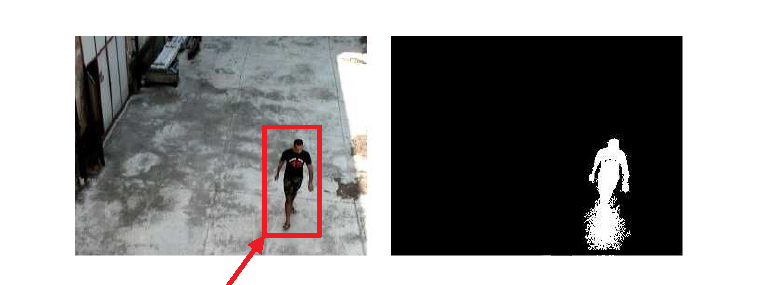
\includegraphics[scale=0.5]{bgsub.png}
\caption[Esempio di background subtraction graduale]{\textit{Esempio di background subtraction graduale. Viene segnalato nella prima finestra quello che è il foreground del video e in seguito nella seconda l'effetto del background subtraction che mette in rilievo il blob bianco rilevato sullo sfondo}\label{fig:bgsub}}
\end{figure}
In letteratura vi sono diversi modelli e metodi per calcolare questa segmentazione tra foreground/background. In particolare citiamo:
\begin{description}
 \item[Distribuzione Unimodale] Il più semplice modello assume che l'intensità del valore di un pixel può essere modellata da una distribuzione unimodale, come una distribuzione Gaussiana $N(\mu,\sigma^2)$
\item [Mixture of Gaussian MOG] Il modello MOG generalizzato viene di solito usato per modelli abbastanza complessi, non statici con molteplici background. Questo tipo di modellazione è di tipo statistico e online. L'idea è quella di modellare ogni pixel in un processo di funzioni gaussiane, successivamente eseguire l'apprendimento online e rilevare il foreground passo passo. In particolare un pixel sarà classificato come un pixel di foreground se la distribuzione a lui associata è stata classificata con minor peso e maggior varianza, viceversa verrà classificato come background pixel.
\item [Tecniche Non Parametriche] Si stima la funziona di densità di probabilità per ogni pixel presi da tanti campioni usando la tecnica di stima sulla densità Kernel.
\item [Approccio basato su regioni o frame]
 \end{description}

Nel nostro applicativo sarà usato il modello di Mixture of Gaussians, in quanto si vuole coprire anche video di una certa complessità e perchè le librerie offrono un buon supporto per questo modello. In particolare ne listato sottostate è visualizzato l'uso di esse nel file adetto al background subtraction.

\lstset{language=c++}
\lstset{commentstyle=\emph}
\begin{lstlisting}[frame=l,caption=Background Subtraction implementato con MOG - getBackground.cpp ,breaklines=true,basicstyle=\small]{Background Subtraction implementato con MOG - getBackground.cpp}


void initBackgroundModel(CvBGStatModel ** bgmodel, IplImage* tmp_frame, CvGaussBGStatModelParams* paramMoG){
	
	paramMoG->win_size = 200; //200;
	paramMoG->n_gauss = 3; //5;
	paramMoG->bg_threshold = 0.1; //0.7;
	paramMoG->std_threshold = 5; //2.5;
	paramMoG->minArea = 200.f; //15.f;
	paramMoG->weight_init = 0.01; //0.05;
	paramMoG->variance_init = 30; //30*30;
	*bgmodel = cvCreateGaussianBGModel(tmp_frame, paramMoG);
	
}


///The function that make the Background subtraction with Gaussian model
/**
 * \param aviName the name of the avi video to process
 * \return savedBackgroundImage the background of the video
 */

IplImage* updateBackground(CvBGStatModel *bg_model, IplImage * tmp_frame){
	 
	//Updating the Gaussian Model

	cvUpdateBGStatModel(tmp_frame, bg_model);
  
	
	//returing the binary background

	return bg_model->foreground;
}


\end{lstlisting}


\subsubsection{Predizione}
\subsubsection{Rappresentazione della predizione}
\subsubsection{HiGui}
\subsubsection{Scripting GNUPlot}

